\documentclass[12pt]{article}
\usepackage{amsmath, amssymb, amsthm, enumerate, graphicx}
\usepackage[usenames,dvipsnames]{color}
\usepackage{bm}
\usepackage[colorlinks=true,urlcolor=blue]{hyperref}
\usepackage{geometry}
\geometry{margin=1in}
\usepackage{float}
\usepackage{graphics}
\setlength{\marginparwidth}{2.15cm}
\usepackage{booktabs}
\usepackage{enumitem}
\usepackage{epsfig}
\usepackage{setspace}
\usepackage{parskip}
\usepackage[normalem]{ulem}
\usepackage{tikz}
\usetikzlibrary{positioning, arrows, automata}
\usepackage{pgfplots}
\usepackage[font=scriptsize]{subcaption}
\usepackage{float}
\usepackage[]{algorithm2e}
\usepackage{environ}
\usepackage{bbm}
\usepackage{titling}
\usepackage{url}
\usepackage{xcolor}
\usepackage{lipsum}
\usepackage{lastpage}
\usepackage[colorlinks=true,urlcolor=blue]{hyperref}
\usepackage{multicol}
\usepackage{tabularx}
\usepackage{comment}
\usepackage[utf8]{inputenc}
\usepackage{amssymb}
\usepackage{setspace}
\usepackage{marvosym}
\usepackage{wrapfig}
\usepackage{datetime}
\usepackage[many]{tcolorbox}
\usepackage{array}
\usepackage{multirow}
\usepackage{wasysym}
\usepackage{cancel}
\usepackage{fancyhdr}
\usepackage{listings}
\usepackage{color}
\usepackage{algorithm}
\usepackage{algorithmicx}
\usepackage[noend]{algpseudocode}

\usepackage{enumitem,amssymb}
\newlist{todolist}{itemize}{2}
\setlist[todolist]{label=$\square$}

\newcommand{\R}{\mathbb{R}}
\newcommand{\blackcircle}{\tikz\draw[black,fill=black] (0,0) circle (1ex);}
\renewcommand{\circle}{\tikz\draw[black] (0,0) circle (1ex);}

\newcommand{\emptysquare}{{\LARGE $\square$}\ \ }
\newcommand{\filledsquare}{{\LARGE $\blacksquare$}\ \ }
\newcommand{\emptycircle}{{\LARGE $\fullmoon$}\ \ }
\newcommand{\filledcircle}{{\LARGE $\newmoon$}\ \ }

\newtcolorbox[]{your_solution}[1][]{
    % breakable,
    enhanced,
    nobeforeafter,
    colback=white,
    title=Your Answer,
    sidebyside align=top,
    box align=top,
    #1
}


%%%%%%%%%%%%%%%%%%%%%%%%%%%%%%%%%%%%%%%%%%
% Custom commands                        %
%%%%%%%%%%%%%%%%%%%%%%%%%%%%%%%%%%%%%%%%%%

\newcommand{\vc}[1]{\boldsymbol{#1}}
\newcommand{\adj}[1]{\frac{d J}{d #1}}
\newcommand{\chain}[2]{\adj{#2} = \adj{#1}\frac{d #1}{d #2}}

% mathcal
\newcommand{\Ac}{\mathcal{A}}
\newcommand{\Bc}{\mathcal{B}}
\newcommand{\Cc}{\mathcal{C}}
\newcommand{\Dc}{\mathcal{D}}
\newcommand{\Ec}{\mathcal{E}}
\newcommand{\Fc}{\mathcal{F}}
\newcommand{\Gc}{\mathcal{G}}
\newcommand{\Hc}{\mathcal{H}}
\newcommand{\Ic}{\mathcal{I}}
\newcommand{\Jc}{\mathcal{J}}
\newcommand{\Kc}{\mathcal{K}}
\newcommand{\Lc}{\mathcal{L}}
\newcommand{\Mc}{\mathcal{M}}
\newcommand{\Nc}{\mathcal{N}}
\newcommand{\Oc}{\mathcal{O}}
\newcommand{\Pc}{\mathcal{P}}
\newcommand{\Qc}{\mathcal{Q}}
\newcommand{\Rc}{\mathcal{R}}
\newcommand{\Sc}{\mathcal{S}}
\newcommand{\Tc}{\mathcal{T}}
\newcommand{\Uc}{\mathcal{U}}
\newcommand{\Vc}{\mathcal{V}}
\newcommand{\Wc}{\mathcal{W}}
\newcommand{\Xc}{\mathcal{X}}
\newcommand{\Yc}{\mathcal{Y}}
\newcommand{\Zc}{\mathcal{Z}}

% mathbb
\newcommand{\Ab}{\mathbb{A}}
\newcommand{\Bb}{\mathbb{B}}
\newcommand{\Cb}{\mathbb{C}}
\newcommand{\Db}{\mathbb{D}}
\newcommand{\Eb}{\mathbb{E}}
\newcommand{\Fb}{\mathbb{F}}
\newcommand{\Gb}{\mathbb{G}}
\newcommand{\Hb}{\mathbb{H}}
\newcommand{\Ib}{\mathbb{I}}
\newcommand{\Jb}{\mathbb{J}}
\newcommand{\Kb}{\mathbb{K}}
\newcommand{\Lb}{\mathbb{L}}
\newcommand{\Mb}{\mathbb{M}}
\newcommand{\Nb}{\mathbb{N}}
\newcommand{\Ob}{\mathbb{O}}
\newcommand{\Pb}{\mathbb{P}}
\newcommand{\Qb}{\mathbb{Q}}
\newcommand{\Rb}{\mathbb{R}}
\newcommand{\Sb}{\mathbb{S}}
\newcommand{\Tb}{\mathbb{T}}
\newcommand{\Ub}{\mathbb{U}}
\newcommand{\Vb}{\mathbb{V}}
\newcommand{\Wb}{\mathbb{W}}
\newcommand{\Xb}{\mathbb{X}}
\newcommand{\Yb}{\mathbb{Y}}
\newcommand{\Zb}{\mathbb{Z}}

% mathbf lowercase
\newcommand{\av}{\mathbf{a}}
\newcommand{\bv}{\mathbf{b}}
\newcommand{\cv}{\mathbf{c}}
\newcommand{\dv}{\mathbf{d}}
\newcommand{\ev}{\mathbf{e}}
\newcommand{\fv}{\mathbf{f}}
\newcommand{\gv}{\mathbf{g}}
\newcommand{\hv}{\mathbf{h}}
\newcommand{\iv}{\mathbf{i}}
\newcommand{\jv}{\mathbf{j}}
\newcommand{\kv}{\mathbf{k}}
\newcommand{\lv}{\mathbf{l}}
\newcommand{\mv}{\mathbf{m}}
\newcommand{\nv}{\mathbf{n}}
\newcommand{\ov}{\mathbf{o}}
\newcommand{\pv}{\mathbf{p}}
\newcommand{\qv}{\mathbf{q}}
\newcommand{\rv}{\mathbf{r}}
\newcommand{\sv}{\mathbf{s}}
\newcommand{\tv}{\mathbf{t}}
\newcommand{\uv}{\mathbf{u}}
\newcommand{\vv}{\mathbf{v}}
\newcommand{\wv}{\mathbf{w}}
\newcommand{\xv}{\mathbf{x}}
\newcommand{\yv}{\mathbf{y}}
\newcommand{\zv}{\mathbf{z}}

% mathbf uppercase
\newcommand{\Av}{\mathbf{A}}
\newcommand{\Bv}{\mathbf{B}}
\newcommand{\Cv}{\mathbf{C}}
\newcommand{\Dv}{\mathbf{D}}
\newcommand{\Ev}{\mathbf{E}}
\newcommand{\Fv}{\mathbf{F}}
\newcommand{\Gv}{\mathbf{G}}
\newcommand{\Hv}{\mathbf{H}}
\newcommand{\Iv}{\mathbf{I}}
\newcommand{\Jv}{\mathbf{J}}
\newcommand{\Kv}{\mathbf{K}}
\newcommand{\Lv}{\mathbf{L}}
\newcommand{\Mv}{\mathbf{M}}
\newcommand{\Nv}{\mathbf{N}}
\newcommand{\Ov}{\mathbf{O}}
\newcommand{\Pv}{\mathbf{P}}
\newcommand{\Qv}{\mathbf{Q}}
\newcommand{\Rv}{\mathbf{R}}
\newcommand{\Sv}{\mathbf{S}}
\newcommand{\Tv}{\mathbf{T}}
\newcommand{\Uv}{\mathbf{U}}
\newcommand{\Vv}{\mathbf{V}}
\newcommand{\Wv}{\mathbf{W}}
\newcommand{\Xv}{\mathbf{X}}
\newcommand{\Yv}{\mathbf{Y}}
\newcommand{\Zv}{\mathbf{Z}}

% bold greek lowercase
\newcommand{\alphav     }{\boldsymbol \alpha     }
\newcommand{\betav      }{\boldsymbol \beta      }
\newcommand{\gammav     }{\boldsymbol \gamma     }
\newcommand{\deltav     }{\boldsymbol \delta     }
\newcommand{\epsilonv   }{\boldsymbol \epsilon   }
\newcommand{\varepsilonv}{\boldsymbol \varepsilon}
\newcommand{\zetav      }{\boldsymbol \zeta      }
\newcommand{\etav       }{\boldsymbol \eta       }
\newcommand{\thetav     }{\boldsymbol \theta     }
\newcommand{\varthetav  }{\boldsymbol \vartheta  }
\newcommand{\iotav      }{\boldsymbol \iota      }
\newcommand{\kappav     }{\boldsymbol \kappa     }
\newcommand{\varkappav  }{\boldsymbol \varkappa  }
\newcommand{\lambdav    }{\boldsymbol \lambda    }
\newcommand{\muv        }{\boldsymbol \mu        }
\newcommand{\nuv        }{\boldsymbol \nu        }
\newcommand{\xiv        }{\boldsymbol \xi        }
\newcommand{\omicronv   }{\boldsymbol \omicron   }
\newcommand{\piv        }{\boldsymbol \pi        }
\newcommand{\varpiv     }{\boldsymbol \varpi     }
\newcommand{\rhov       }{\boldsymbol \rho       }
\newcommand{\varrhov    }{\boldsymbol \varrho    }
\newcommand{\sigmav     }{\boldsymbol \sigma     }
\newcommand{\varsigmav  }{\boldsymbol \varsigma  }
\newcommand{\tauv       }{\boldsymbol \tau       }
\newcommand{\upsilonv   }{\boldsymbol \upsilon   }
\newcommand{\phiv       }{\boldsymbol \phi       }
\newcommand{\varphiv    }{\boldsymbol \varphi    }
\newcommand{\chiv       }{\boldsymbol \chi       }
\newcommand{\psiv       }{\boldsymbol \psi       }
\newcommand{\omegav     }{\boldsymbol \omega     }

% bold greek uppercase
\newcommand{\Gammav     }{\boldsymbol \Gamma     }
\newcommand{\Deltav     }{\boldsymbol \Delta     }
\newcommand{\Thetav     }{\boldsymbol \Theta     }
\newcommand{\Lambdav    }{\boldsymbol \Lambda    }
\newcommand{\Xiv        }{\boldsymbol \Xi        }
\newcommand{\Piv        }{\boldsymbol \Pi        }
\newcommand{\Sigmav     }{\boldsymbol \Sigma     }
\newcommand{\Upsilonv   }{\boldsymbol \Upsilon   }
\newcommand{\Phiv       }{\boldsymbol \Phi       }
\newcommand{\Psiv       }{\boldsymbol \Psi       }
\newcommand{\Omegav     }{\boldsymbol \Omega     }


% SOLUTION environment
\NewEnviron{soln}{
\leavevmode\color{red}\ignorespaces \textbf{SOL:} \BODY
% \leavevmode\color{white}\ignorespaces \textbf{Solution} \BODY
}{}

% QUESTION AUTHORS environment
\NewEnviron{qauthor}{
\leavevmode\color{blue}\ignorespaces \textbf{Author} \BODY
% \leavevmode\color{white}\ignorespaces \textbf{Author} \BODY
}{}


%\newcommand{\norm}[1]{\lVert #1 \rVert}
%\newcommand{\st}{\mathrm{s.t.}}

\makeatletter
\newcommand{\removelatexerror}{\let\@latex@error\@gobble}
\makeatother

\newcommand{\argmax}{\mathop{\mathrm{argmax}}}
\newcommand{\argmin}{\mathop{\mathrm{argmin}}}


%%%%%%%%%%%%%%%%%%%%%%%%%%%%%%%%%%%%%%%%%%%
% Custom box for highlights               %
%%%%%%%%%%%%%%%%%%%%%%%%%%%%%%%%%%%%%%%%%%%

% Define box and box title style
\tikzstyle{mybox} = [fill=blue!10, very thick,
    rectangle, rounded corners, inner sep=1em, inner ysep=1em]

% \newcommand{\notebox}[1]{
% \begin{tikzpicture}
% \node [mybox] (box){%
%     \begin{minipage}{\textwidth}
%     #1
%     \end{minipage}
% };
% \end{tikzpicture}%
% }

\NewEnviron{notebox}{
\begin{tikzpicture}
\node [mybox] (box){
    \begin{minipage}{\textwidth}
        \BODY
    \end{minipage}
};
\end{tikzpicture}
}


\begin{document}

\section*{}
\begin{center}
  \centerline{\textsc{\LARGE  Homework 3}}
  \vspace{0.5em}
  \centerline{\textsc{\large KNNs, SVMs and Neural Networks}}% \footnote{Compiled on \today{} at \currenttime{}}}
  \vspace{1em}
  \textsc{\large CMU 10-701: Machine Learning (Spring 2022)} \\
  \vspace{0.5em}
  \url{piazza.com/cmu/spring2022/10701/home} \\
  \vspace{0.5em}
  \centerline{OUT: Thursday, March 03, 2022}
  %\today{} at \currenttime{}}}
  \vspace{0.5em}
  \centerline{\textbf{DUE: Wednesday, March 23, 2022, 11:59pm}}
\end{center}

\section*{START HERE: Instructions}
\begin{itemize}
\item \textbf{Collaboration policy:} Collaboration on solving the homework is allowed, after you have thought about the problems on your own. It is also OK to get clarification (but not solutions) from books or online resources, again after you have thought about the problems on your own. There are two requirements: first, cite your collaborators fully and completely (e.g., ``Jane explained to me what is asked in Question 2.1''). Second, write your solution {\em independently}: close the book and all of your notes, and send collaborators out of the room, so that the solution comes from you only.  See the Academic Integrity Section in our course syllabus for more information: \url{https://piazza.com/class_profile/get_resource/ksetdrgdkob78/ksqc9bxxjt56ic}

\item\textbf{Late Submission Policy:} See the late submission policy here: \url{https://piazza.com/class_profile/get_resource/ksetdrgdkob78/ksqc9bxxjt56ic}

\item\textbf{Submitting your work:} 

\begin{itemize}

\item \textbf{Gradescope:} There will be two submission slots for this homework on Gradescope: Written and Programming. \\
For the written problems such as short answer, multiple choice, derivations, proofs, or plots, we will be using the written submission slot. Please use the provided template. The best way to format your homework is by using the Latex template released in the handout and writing your solutions in Latex. However submissions can be handwritten onto the template, but should be labeled and clearly legible. If your writing is not legible, you will not be awarded marks.  Each derivation/proof should be  completed in the boxes provided below the question, \textbf{you should not move or change the sizes of these boxes} as Gradescope is expecting your solved homework PDF to match the template on Gradescope. If you find you need more space than the box provides you should consider cutting your solution down to its relevant parts, if you see no way to do this, please add an additional page at the end of the homework and guide us there with a 'See page xx for the rest of the solution'.\\
You are also required to upload your code, which you wrote to solve the final question of this homework, to the Programming submission slot. Your code may be run by TAs so please make sure it is in a workable state.\\
Regrade requests can be made after the homework grades are released, however this gives the TA the opportunity to regrade your entire paper, meaning if additional mistakes are found then points will be deducted. 
\end{itemize}

\end{itemize}

For multiple choice or select all that apply questions, shade in the box or circle in the template document corresponding to the correct answer(s) for each of the questions. For \LaTeX users, use $\blacksquare$ and \blackcircle  for shaded boxes and circles, and don't change anything else. If an answer box is included for showing work, \textbf{you must show your work}!


\clearpage
\section*{Problem 1: K-Nearest Neighbors - Black Box [10 Points]}

\begin{enumerate}

        \item \textbf{[6 pts]} In a KNN classification problem, assume that the distance measure is not explicitly specified to you. Instead, you are given a “black box” where you input a set of instances $P_1, P_2, \dots P_n$ and a new example $Q$, and the black box outputs the nearest neighbor of $Q$, say $P_i$ and its corresponding class label $C_i$. Is it possible to construct a KNN classification algorithm (w.r.t the unknown distance metrics) based on this black box alone? If so, how and if not, why not?
        \begin{tcolorbox}[fit,height=7cm, width=0.9\textwidth, blank, borderline={1pt}{-2pt}]
        %solution 
        \end{tcolorbox}
        
        \item \textbf{[4 pts]} If the black box returns the $j$ nearest neighbors (and their corresponding class labels) instead of the single most nearest neighbor (assume $j \neq k$), is it possible to construct a KNN classification algorithm based on the black box? If so how, and if not why not?
        \begin{tcolorbox}[fit,height=7cm, width=0.9\textwidth, blank, borderline={1pt}{-2pt}]
        %solution 
        \end{tcolorbox}
    

    \clearpage
\end{enumerate}

\clearpage
\section*{Problem 2: Soft Margin Hyperplanes [9 points]}
The soft-margin primal SVM problem is:

\begin{align}\label{eqn:soft-svm}\text{min} \frac{1}{2} ||\textbf{w}||_2^2 + C \sum_{i=1}^N \xi^{(i)} \end{align}

subject to feasibility constraints that for all $i=1,...,N$:

$$y^{(i)}(\textbf{w}^T \xv^{(i)} + b) \geq 1 - \xi^{(i)}$$
$$\xi^{(i)} \geq 0$$

Suppose instead the optimization objective was  changed to $\frac{1}{2}||\textbf{w}||_2^2 + C \sum_{i=1}^N \xi^{(i)}^2$ while the feasibility constraints are kept the same. 

\textbf{Hint}: Before attempting this problem, we highly recommend first trying to derive the dual formulations for the hard-margin and soft-margin SVMs presented in class by working through the steps detailed below.

\begin{enumerate}
\item \textbf{[2pts]} \textbf{Short Answer: }
         How is the penalty changed (relative to the original formulation \ref{eqn:soft-svm}) for points within the margin? How about misclassified points?
        
 
    \begin{tcolorbox}[fit,height=4cm, width=15cm, blank, borderline={1pt}{-2pt},nobeforeafter]
        %solution
    \end{tcolorbox}
    
    
\item \textbf{[1 pt]} Incorporate the feasibility constraints into the objective function using the method of Lagrange multipliers by writing out the Lagrangian and the associated constraints. 

\begin{tcolorbox}[fit,height=5.0cm, width=0.95\textwidth, blank, borderline={1pt}{-2pt}]
%solution 
\end{tcolorbox}

% \newpage 

\item \textbf{[3 pts]} Next, take the partial derivative of the Lagrangian with respect to all of the optimization variables. Be sure to show all of you work.

\begin{tcolorbox}[fit,height=21.0cm, width=0.95\textwidth, blank, borderline={1pt}{-2pt}]
%solution 
\end{tcolorbox}

\newpage
\item \textbf{[3 pts]} Finally, by setting the partial derivatives from the previous part equal to 0, derive the dual formulation of SVMs in this general case. Again, be sure to show all of you work.


\begin{tcolorbox}[fit,height=18.0cm, width=0.95\textwidth, blank, borderline={1pt}{-2pt}]
%solution 
\end{tcolorbox}

\end{enumerate}







\clearpage
\section*{Problem 3: Neural Nets: Written Questions [30 pts]}
\label{sec:written}

\textbf{Note:} We strongly encourage you to do the written part of this homework before the programming, as it will help you gain familiarity with the calculations you will have to code up in the programming section. We suggest that for each of these problems, you write out the equation required to calculate each value in terms of the variables we created ($a_j, z_j, b_k$, etc.) before you calculate the numerical value.

\textbf{Note:} For all questions which require numerical answers, round up your final answers to four decimal places. For integers, you may drop trailing zeros. We will use column vectors for the data and neural network layers, be consistent with the question in your answers involving vectors. If your answer involves application of an operator element-wise to a vector or a matrix, state it explicitly.

 \begin{figure}[h]
        \centering
        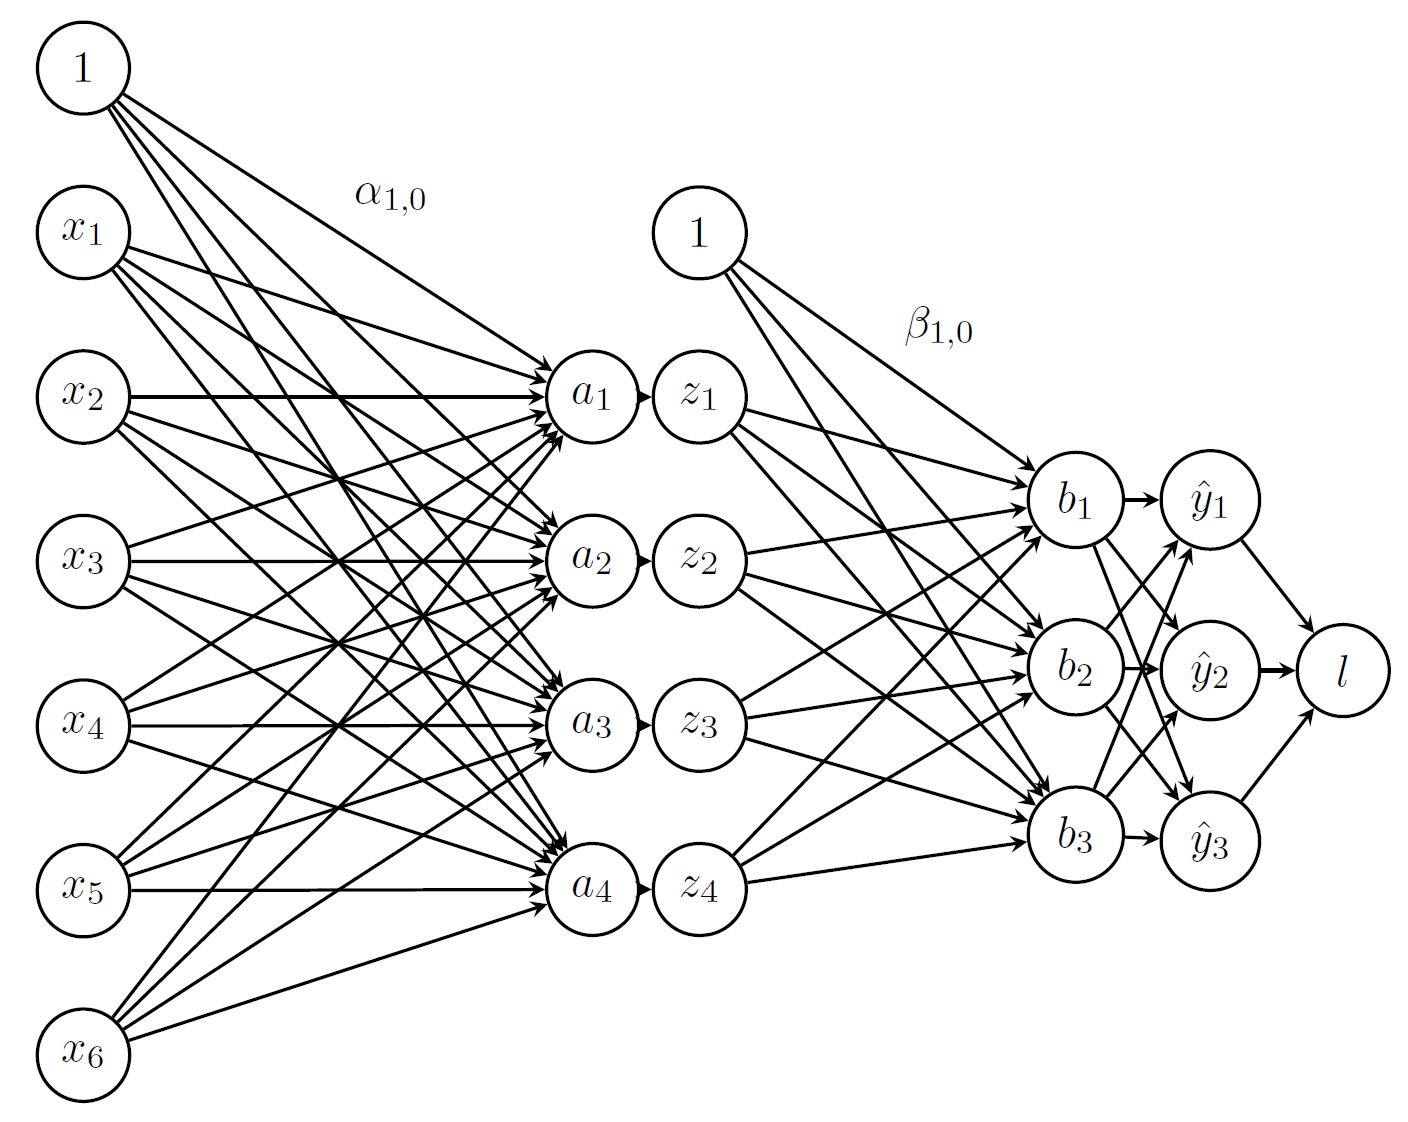
\includegraphics[height=9cm]{img/network.png}
        \caption{A One Hidden Layer Neural Network}
        \label{fig:oneHL}
    \end{figure}

\subsubsection*{\textcolor{purple}{Network Overview}}
Consider the neural network with one hidden layer shown in Figure \ref{fig:oneHL}. The input layer consists of 6 features $\xv = [x_1,...,x_6]^T$, the hidden layer has 4  nodes $\zv = [z_1,...,z_4]^T$, and the output layer is $\hat{\yv} = [\hat{y}_1, \hat{y}_2, \hat{y}_3]^T$ that sums to one over 3 classes. We also add a bias to the input, $x_0 = 1$ and the hidden layer $z_0 = 1$, both of which are fixed to $1$.


We adopt the following notation:
\begin{enumerate}
    \item Let \textcolor{magenta}{$\boldsymbol{\alpha}$} be the matrix of weights from the inputs to the hidden layer.
    \item Let \textcolor{magenta}{$\boldsymbol{\beta}$} be the matrix of weights from the hidden layer to the output layer.
    \item Let \textcolor{magenta}{$\alpha_{j,i}$} represent the weight going \textit{to} the node $z_j$ in the hidden layer \textit{from} the node $x_i$ in the input layer (e.g. $\alpha_{1,2}$ is the weight from $x_2$ to $z_1$)
    \item Let \textcolor{magenta}{$\boldsymbol{\beta}_{k,j}$} represent the weight going \textit{to} the node $y_k$ in the output layer \textit{from} the node $z_j$ in the hidden layer.
    \item We will use a \emph{sigmoid activation function (\textcolor{magenta}{$\sigma$})} for the hidden layer and a \emph{softmax} for the output layer. 
\end{enumerate}

\subsubsection*{\textcolor{purple}{Network Details}}
Equivalently, we define each of the following. 

The input:
\begin{align}
\xv=[x_1,x_2,x_3,x_4,x_5,x_6]^T
\end{align}

Linear combination at first (hidden) layer:
\begin{equation}
a_j= \alpha_{j,0} + \sum_{i=1}^6 \alpha_{j,i}x_i,\quad j \in \{1,\ldots,4\}
\end{equation}

Activation at first (hidden) layer:
\begin{align}
z_j &= \sigma(a_j) = \frac{1}{1+\exp(-a_j)},\quad  j \in \{1,\ldots,4\}
\end{align}

Linear combination at second (output) layer:
\begin{equation}
b_k = \beta_{k,0} + \sum_{j=1}^4 \beta_{k,j}z_j,\quad  k \in \{1,\ldots,3\}
\end{equation}

Activation at second (output) layer:
\begin{equation}
\hat{y}_k = \frac{\exp(b_k)}{\sum\limits_{l=1}^3 \exp(b_l)},\quad  k \in \{1,\ldots,3\}
\end{equation}

Note that the linear combination equations can be written equivalently as the product of the weight matrix with the input vector. We can even fold in the bias term $\alpha_0$ by thinking of $x_0 = 1$, and fold in $\beta_0$ by thinking of $z_0 = 1$.

\subsubsection*{\textcolor{purple}{Loss}}

We will use cross entropy loss, $\ell(\hat{\yv},\yv)$. If $\yv$ represents our target (true) output, which will be a \textcolor{purple}{one-hot vector} representing the correct class, and $\hat{\yv}$ represents the output of the network, the loss is calculated as (note that the $\log$ terms are in base $e$):
\begin{equation}
   \ell(\hat{\yv},\yv) = - \sum_{k=1}^3 y_k \log(\hat{y}_k)
\end{equation}
%%%%%%%%%%%%%%%%%%%%

\begin{enumerate}
\item \textbf{[6 pts]} In the following questions you will derive the matrix and vector forms of the previous equations which define our neural network. These are what you should hope to program in order to avoid excessive loops and large run times.\\
When working these out it is important to keep a note of the vector and matrix dimensions in order for you to easily identify what is and isn't a valid multiplication. Suppose you are given a training example: $\xv^{(1)}=[x_1,x_2,x_3,x_4,x_5,x_6]^T$ with \textbf{label class 2}, so $\yv^{(1)}=[0,1,0]^T$. We initialize the network weights as:
\begin{center}
$$\boldsymbol{\alpha^*}=
    \begin{bmatrix}
    \alpha_{1,1} & \alpha_{1,2} & \alpha_{1,3} & \alpha_{1,4} & \alpha_{1,5} & \alpha_{1,6} \\
    \alpha_{2,1} & \alpha_{2,2} & \alpha_{2,3} & \alpha_{2,4} & \alpha_{2,5} & \alpha_{2,6} \\
    \alpha_{3,1} & \alpha_{3,2} & \alpha_{3,3} & \alpha_{3,4} & \alpha_{3,5} & \alpha_{3,6} \\
    \alpha_{4,1} & \alpha_{4,2} & \alpha_{4,3} & \alpha_{4,4} & \alpha_{4,5} & \alpha_{4,6}
    \end{bmatrix}$$
    
$$\boldsymbol{\beta^*}=
    \begin{bmatrix}
    \beta_{1,1} & \beta_{1,2} & \beta_{1,3} & \beta_{1,4} \\
    \beta_{2,1} & \beta_{2,2} & \beta_{2,3} & \beta_{2,4} \\
    \beta_{3,1} & \beta_{3,2} & \beta_{3,3} & \beta_{3,4}
    \end{bmatrix}
$$
\end{center}
    
We want to also consider the bias term and the weights on the bias terms (${\alpha}_{j,0}$ and ${\beta}_{k,0})$. To account for these we can add a new column to the beginning of our initial weight matrices. 

$$\boldsymbol{\alpha}=
    \begin{bmatrix}
    \textcolor{blue}{\alpha_{1,0}} & \alpha_{1,1} & \alpha_{1,2} & \alpha_{1,3} & \alpha_{1,4} & \alpha_{1,5} & \alpha_{1,6} \\
    \textcolor{blue}{\alpha_{2,0}} & \alpha_{2,1} & \alpha_{2,2} & \alpha_{2,3} & \alpha_{2,4} & \alpha_{2,5} & \alpha_{2,6} \\
    \textcolor{blue}{\alpha_{3,0}} & \alpha_{3,1} & \alpha_{3,2} & \alpha_{3,3} & \alpha_{3,4} & \alpha_{3,5} & \alpha_{3,6} \\
    \textcolor{blue}{\alpha_{4,0}} & \alpha_{4,1} & \alpha_{4,2} & \alpha_{4,0} & \alpha_{4,4} & \alpha_{4,5} & \alpha_{4,6}
    \end{bmatrix}$$
    
$$\boldsymbol{\beta}=
    \begin{bmatrix}
    \textcolor{blue}{\beta_{1,0}} & \beta_{1,1} & \beta_{1,2} & \beta_{1,3} & \beta_{1,4} \\
    \textcolor{blue}{\beta_{2,0}} & \beta_{2,1} & \beta_{2,2} & \beta_{2,3} & \beta_{2,4} \\
    \textcolor{blue}{\beta_{3,0}} & \beta_{3,1} & \beta_{3,2} & \beta_{3,3} & \beta_{3,4}
    \end{bmatrix}$$

    And we can set our first value of our input vectors to always be 1 ($x_0^{(i)} = 1$), so our input becomes: $$\xv^{(1)}=[\textcolor{blue}{1},x_1,x_2,x_3,x_4,x_5,x_6]^T$$
    
    
    \begin{enumerate}
        \item \textbf{[1 pt]} By examining the shapes of the initial weight matrices, how many neurons (or nodes) do we have in the first hidden layer of the neural network? (Not including the bias neuron)
        
        \begin{tcolorbox}[fit,height=1cm, width=2cm, blank, borderline={1pt}{-2pt}]
            %solution 
        \end{tcolorbox}

        
        
        
        \item \textbf{[1 pt]} How many output neurons will our neural network have?
        
        \begin{tcolorbox}[fit,height=1cm, width=2cm, blank, borderline={1pt}{-2pt}]
            %solution 
        \end{tcolorbox}

        
        
        
        
        \item \textbf{[1 pt]} What is the vector $\av$ whose elements are made up of the entries $a_j$ in equation (4). Write your answer in terms of $\alphav$ and $\xv^{(1)}$.
        
        
        \begin{tcolorbox}[fit,height=1cm, width=4cm, blank, borderline={1pt}{-2pt}]
            %solution 
        \end{tcolorbox}
        
        
        
        
        \item \textbf{[1 pt]} What is the vector $\zv$ whose elements are made up of the entries $z_j$ in equation (5)? Write your answer in terms of $\av$.
        
        \begin{tcolorbox}[fit,height=2cm, width=14cm, blank, borderline={1pt}{-2pt}]
            %solution 
        \end{tcolorbox}

        
        \item \textbf{[1 pt]} \textbf{Select one:} We cannot take the matrix multiplication of our weights $\betav$ and our vector $\zv$ since they are not compatible shapes. Which of the following would allow us to take the matrix multiplication of $\betav$ and $\zv$ such that the entries of the vector $\bv = \betav\zv$ are equivalent to the values of $b_k$ in equation (5)? 
        
        \begin{list}{}
        \item $\circle$ Remove the last column of $\betav$
        \item $\circle$ Remove the first row of $\zv$
        \item $\circle$ Append a value of 1 to be the first entry of $\zv$
        \item $\circle$ Append an additional column of 1's to be the first column of $\betav$ 
        \item $\circle$ Append a row of 1's to be the first row of $\betav$ 
        \item $\circle$ Take the transpose of $\betav$
        \end{list}
        
        
        
        \item \textbf{[1 pt]} What are the entries of the output vector $\hat{\yv}$? Your answer should be written in terms of $b_1,b_2,b_3$.
        
        \begin{tcolorbox}[fit,height=3.3cm, width=14cm, blank, borderline={1pt}{-2pt}]
            %solution 
        \end{tcolorbox}
        
        
    \end{enumerate} 

\item \textbf{[7 pts]} We will now derive the matrix and vector forms for the backpropagation algorithm.

$$\frac{d\ell}{d\alphav} = 
    \begin{bmatrix}
        \adj{\alpha_{10}} & \adj{\alpha_{11}} & \dots  & \adj{\alpha_{1M}} \\
        \adj{\alpha_{20}} & \adj{\alpha_{21}} & \dots  & \adj{\alpha_{2M}} \\
        \vdots      & \vdots      & \ddots & \vdots \\
        \adj{\alpha_{D0}} & \adj{\alpha_{D1}} & \dots  & \adj{\alpha_{DM}}
    \end{bmatrix}$$




The mathematics which you have to derive in this section jump significantly in difficultly, you should always be examining the shape of the matrices and vectors and making sure that you are comparing your matrix elements with calculations of individual derivatives to make sure they match (e.g. the element of the matrix $(\frac{d\ell}{d\alpha})_{2,1}$ should be equal to $\frac{d\ell}{d\alpha_{2,1}}$  ). Recall that $\ell$ is our loss function defined in equation (1.8)
    
    \begin{enumerate}
        \item \textbf{[1 pt]} The derivative of the softmax function with respect to $b_k$ is as follows:
        $$\frac{d\hat{y}_l}{db_k} = \hat{y}_l(\Ib[k=l]-\hat{y}_k)$$ 
        where $\Ib[k=l]$ is an indicator function such that if $k=l$ then it it returns value 1 and 0 otherwise. 
        Using this, write the derivative $\frac{d\ell}{db_k}$ in a smart way such that you do not need this indicator function. Write your solutions in terms of $\hat{y}_k,y_k$.
        
        
        \begin{tcolorbox}[fit,height=2cm, width=12cm, blank, borderline={1pt}{-2pt}]
            %solution 
        \end{tcolorbox}
        
        
        \item \textbf{[1 pt]} What are the elements of the vector $\frac{d\ell}{db}$? (Recall that  $\yv^{(1)}=[0,1,0]^T$)
        
        
        \begin{tcolorbox}[fit,height=1cm, width=6cm, blank, borderline={1pt}{-2pt}]
            %solution 
        \end{tcolorbox}
        
        
        
        \item \textbf{[1 pt]} What is the derivative $\frac{d\ell}{d\beta}$? Your answer should be in terms of $\frac{d\ell}{d\bv}$ and $\zv$.
        
        
        \begin{tcolorbox}[fit,height=3cm, width=12cm, blank, borderline={1pt}{-2pt}]
            %solution 
        \end{tcolorbox}
        
        
        
        \item \textbf{[1 pt]} Explain in one short sentance why must we go back to using the matrix $\betav^*$ (The matrix $\betav$ without the first column of ones) when calculating the matrix $\frac{d\ell}{d\alpha}$?
        
        
        \begin{tcolorbox}[fit,height=1cm, width=15cm, blank, borderline={1pt}{-2pt}]
            %solution 
        \end{tcolorbox}
        
        
        
        \item \textbf{[1 pt]} What is the derivative $\frac{d\ell}{d\zv}$? Your answer should be in terms of $\frac{d\ell}{d\bv}$ and $\betav^*$
        
        
        \begin{tcolorbox}[fit,height=3cm, width=12cm, blank, borderline={1pt}{-2pt}]
            %solution 
        \end{tcolorbox}
        
        
        \item \textbf{[1 pt]} What is the derivative $\frac{d\ell}{d\av}$ in terms of $\frac{d\ell}{d\zv}$ and $\zv$?
        
        
        \begin{tcolorbox}[fit,height=3cm, width=12cm, blank, borderline={1pt}{-2pt}]
            %solution 
        \end{tcolorbox}
        
        
        \item \textbf{[1 pt]} What is the matrix $\frac{d\ell}{d\alpha}$? Your answer should be in terms of $\frac{d\ell}{d\av}$ and $x^{(1)}$.
        
        
        \begin{tcolorbox}[fit,height=3cm, width=12cm, blank, borderline={1pt}{-2pt}]
            %solution 
        \end{tcolorbox}

\end{enumerate}



%%%%%%%%%%%%%%%%%%%%%%%%
\newpage
\subsubsection*{\textcolor{purple}{Prediction}}
When doing prediction, we will predict the \textcolor{purple}{$\argmax$} of the output layer. For example, if $\hat{\yv}$ is such that $\hat{y}_1=0.3,~ \hat{y}_2=0.2,~ \hat{y}_3=0.5$ we would predict class 3 for the input $\xv$. If the true class from the training data $\xv$ was $2$ we would have a \textcolor{purple}{one-hot vector} $\yv$ with values $y_1=0$,~ $y_2=1$,~ $y_3=0$.
    
\item \textcolor{black}{\textbf{[8 pts]}}
     We initialize the weights as:
\begin{center}
$$\boldsymbol{\alpha^*}=
    \begin{bmatrix}
    2 & 1 & -1 & -1 & 0 & -2 \\
    0 & 1 & 0 & -1 & 1 & 3 \\
    -1 & 2 & 1 & 3 & 1 & -1 \\
    1 & 3 & 4 & 2 & -1 & 2
    \end{bmatrix}$$
$$\boldsymbol{\beta^*}=
    \begin{bmatrix}
    2 & -2 & 2 & 1 \\
    3 & -1 & 1 & 2 \\
    0 & -1 & 0 & 1
    \end{bmatrix}
$$
\end{center}
    
And weights on the bias terms (${\alpha}_{j,0}$ and ${\beta}_{j,0})$ are initialized to 1.
    
    You are given a training example $\xv^{(1)}=[1,0,1,0,1,0]^T$ with label class 2, so $\yv^{(1)}=[0,1,0]^T$. Using the initial weights, run the feed forward of the network over this training example (without rounding during the calculation) and then answer the following questions. 
    %In your responses, round to four decimal places---if the answer is an integer you need not include trailing zeros. 
    
    \begin{enumerate}
        \item \textbf{[1 pt]} What is the value of $a_1$?
        
        \begin{tcolorbox}[fit,height=1cm, width=2cm, blank, borderline={1pt}{-2pt}]
            %solution 
        \end{tcolorbox}
        
        \item \textbf{[1 pt]} What is the value of $z_1$?
        
        \begin{tcolorbox}[fit,height=1cm, width=2cm, blank, borderline={1pt}{-2pt}]
         %solution 
        \end{tcolorbox}
        
        \item \textbf{[1 pt]} What is the value of $a_3$?
        
        \begin{tcolorbox}[fit,height=1cm, width=2cm, blank, borderline={1pt}{-2pt}]
        %solution 
        \end{tcolorbox}
        
        \item \textbf{[1 pt]} What is the value of $z_3$?
        
        \begin{tcolorbox}[fit,height=1cm, width=2cm, blank, borderline={1pt}{-2pt}]
            %solution 
        \end{tcolorbox}
        
        \item \textbf{[1 pt]} What is the value of $b_2$?
        
        \begin{tcolorbox}[fit,height=1cm, width=2cm, blank, borderline={1pt}{-2pt}]
            %solution 
        \end{tcolorbox}
        
        \item \textbf{[1 pt]} What is the value of $\hat{y}_2$?
        
        \begin{tcolorbox}[fit,height=1cm, width=2cm, blank, borderline={1pt}{-2pt}]
            %solution 
        \end{tcolorbox}
        
        \item \textbf{[1 pt]} Which class value we would predict on this training example?
        
        \begin{tcolorbox}[fit,height=1cm, width=2cm, blank, borderline={1pt}{-2pt}]
            %solution 
        \end{tcolorbox}

        \item \textbf{[1 pt]} What is the value of the total loss on this training example?
        
        \begin{tcolorbox}[fit,height=1cm, width=2cm, blank, borderline={1pt}{-2pt}]
            %solution 
        \end{tcolorbox}
        
    \end{enumerate}
    
  %  \clearpage
\item \textcolor{black}{\textbf{[4 pts]}} Now use the results of the previous question to run backpropagation over the network and update the weights. Use the learning rate $\eta=1$. 
    
    Do your backpropagation calculations without any rounding then answer the following questions: (in your final responses round to four decimal places)
    
     \begin{enumerate}
        \item \textbf{[1 pt]} What is the updated value of ${\beta}_{2,1}$?
        
        \begin{tcolorbox}[fit,height=1cm, width=2cm, blank, borderline={1pt}{-2pt}]
            %solution 
        \end{tcolorbox}
        
        \item \textbf{[1 pt]} What is the updated weight of the hidden layer bias term applied to $y_1$ (i.e. ${\beta}_{1,0}$)?
        
        \begin{tcolorbox}[fit,height=1cm, width=2cm, blank, borderline={1pt}{-2pt}]
            %solution 
        \end{tcolorbox}
        
        \item \textbf{[1 pt]} What is the updated value of ${\alpha}_{3,4}$?
        
        \begin{tcolorbox}[fit,height=1cm, width=2cm, blank, borderline={1pt}{-2pt}]
            %solution 
        \end{tcolorbox}
        
        \item \textbf{[1 pt]} If we ran backpropagation on this example for a large number of iterations and then ran feed forward over the same example again, which class would we predict?
        
        \begin{tcolorbox}[fit,height=1cm, width=2cm, blank, borderline={1pt}{-2pt}]
            %solution 
        \end{tcolorbox}
        
    \end{enumerate}

\clearpage
\item \textcolor{black}{\textbf{[5 pts]}} Let us now regularize the weights in our neural network. For this question, we will incorporate L2 regularization into our loss function $\ell(\hat{\yv},\yv)$, with the parameter $\lambda$ controlling the weight given to the regularization term. 
\begin{enumerate}
    \item \textbf{[1 pt]} Write the expression for the regularized loss function of our network after adding L2 regularization (\textbf{Hint:} Remember that bias terms should not be regularized!) 
    \begin{tcolorbox}[fit,height=3cm, width=15cm, blank, borderline={1pt}{-2pt}]
            %solution 
    \end{tcolorbox}
        
    \item \textbf{[1 pts]} Compute the regularized loss for training example $\xv^{(1)}$ (assume $\lambda$ = 0.01 and use the weights before backpropagation)
    \begin{tcolorbox}[fit,height=1cm, width=2cm, blank, borderline={1pt}{-2pt}]
            %solution 
    \end{tcolorbox}
    
     \item \textbf{[1 pts]} For a network which uses the regularized loss function, write the gradient update equation for $\alpha_{j,i}$ . You may use $\frac{\partial \ell(\hat{\yv},\yv)}{\partial \alpha_{j,i}}$ to denote the gradient update w.r.t non-regularized loss and $\eta$ to denote the learning rate.
    \begin{tcolorbox}[fit,height=3cm, width=15cm, blank, borderline={1pt}{-2pt}]
            %solution 
    \end{tcolorbox}
    
    
    \item \textbf{[2 pts]} Based on your observations from previous questions, \textbf{select all statements which are true}:
    \begin{list}{}
    \item $\square$ The non-regularized loss is always higher than the regularized loss 
    \item $\square$ As weights become larger, the regularized loss increases faster than non-regularized loss
    \item $\square$ On adding regularization to the loss function, gradient updates for the network become larger
    \item $\square$ When using large initial weights, weight values decrease more rapidly for a network which uses regularized loss 
    \item $\square$ None of the above
    \end{list}
    
\end{enumerate}
\end{enumerate}

\clearpage

\section*{Problem 4: Neural Network Implementation [51 pts]}
\label{sec:code}

\begin{figure}[H]
    \centering
    
\includegraphics[scale=0.99]{img/10lettergrid.png}
    \caption{10 Random Images of Each of 10 Letters in OCR}
    \label{fig:grid}
\end{figure}

Your goal in this assignment is to label images of handwritten letters by implementing a Neural Network from scratch. You will implement all of the functions needed to initialize, train, evaluate, and make predictions with the network. 

\subsection{The Task and Datasets}
\label{sec:dataset}

\subsubsection*{Datasets} We will be using a subset of an Optical Character Recognition (OCR) dataset. This data includes images of all 26 handwritten letters; our subset will include only the letters ``a," ``e," ``g," ``i," ``l," ``n," ``o," ``r," ``t," and ``u."  The handout contains three datasets drawn from this data: a small dataset with 60 samples per class (50 for training and 10 for \ntset), a medium dataset with 600 samples per class (500 for training and 100 for \ntset), and a large dataset with 1000 samples per class (900 for training and 100 for \ntset). Figure \ref{fig:grid} shows a random sample of 10 images of few letters from the dataset.

\subsubsection*{File Format} Each dataset (small, medium, and large) consists of two csv files---train and \ntset. Each row contains 129 columns separated by commas. The first column contains the label and columns 2 to 129 represent the pixel values of a $16 \times 8$ image in a row major format. Label 0 corresponds to ``a," 1 to ``e," 2 to ``g," 3 to ``i," 4 to ``l," 5 to ``n," 6 to ``o," 7 to ``r," 8 to ``t," and 9 to ``u."
%
Because the original images are black-and-white (not grayscale), the pixel values are either 0 or 1. However, you should write your code to accept arbitrary pixel values in the range [0,1]. The images in Figure \ref{fig:grid} were produced by converting these pixel values into .png files for visualization. Observe that no feature engineering has been done here; instead the neural network you build will \emph{learn} features appropriate for the task of character recognition.


\subsection{Model Definition}

In this assignment, you will implement a single-hidden-layer neural network with a sigmoid activation function for the hidden layer, and a softmax on the output layer. Let the input vectors $\xv$ be of length $M$, the hidden layer $\zv$ consist of $D$ hidden units, and the output layer $\hat{\yv}$ be a probability distribution over $K$ classes. That is, each element $y^k$ of the output vector represents the probability of $\xv$ belonging to the class $k$. 
\\\\\begin{center}
    
\begin{tabular}{ |p{3cm}|p{4cm}|p{3cm}|  }
\hline
\multicolumn{3}{|c|}{Model Architecture} \\
\hline
Input (length) & Layer/Activation & Output (length) \\
\hline
\textbf{x} of length $M$ & Linear (hidden layer) & \textbf{a} of length $D$ \\
\textbf{a} of length $D$ & Sigmoid Activation   & \textbf{z} of length $D$ \\
\textbf{z} of length $D$ & Linear (output layer) & \textbf{b} of length $K$ \\
\textbf{b} of length $K$  & Softmax & \textbf{y} of length $K$ \\
\hline
\end{tabular}
\end{center}\par
\vspace{0.2in}
We can further express this model by adding bias features to the inputs of layers; assume $x^0=1$ is a bias feature on the input and that $z^0=1$ is also fixed. In this way, we have two parameter matrices $\alphav \in \Rb^{D \times (M+1)}$ and $\betav \in \Rb^{K \times (D+1)}$. The extra $0$th column of each matrix (i.e. $\alphav^{\cdot,0}$ and $\betav^{\cdot,0}$) hold the bias parameters. Remember to add the appropriate 0th columns to your inputs/matrices and update the dimensions accordingly (i.e. length $D+1$ instead of $D$). 

\begin{align*}
& a^j = \sum_{m=0}^M \alpha^{jm} x^m \\
& z^j = \frac{1}{1+\exp(-a^j)} \\
& b^k =  \sum_{j=0}^D \beta^{kj} z^j\\
& \hat{y}^k = \frac{\exp(b^k)}{\sum_{l=1}^K \exp(b^l)}\\
\end{align*}
The objective function we're using is the average cross entropy over the training dataset $\Dc = \{ (\xv^{(i)}, \yv^{(i)}) \}$:

\begin{align*}
J(\alphav, \betav)= - \frac{1}{N} \sum_{i=1}^N \sum_{k=1}^{K} y^{(i)^k} \log (\hat{y}^{(i)^k})
\end{align*}

Some points to mention:
\begin{itemize}
\item Do \emph{not} use any machine learning libraries. You may and please do use NumPy.
\item Try to ``vectorize'' your code as much as possible. In Python, you want to avoid for-loops and instead rely on \lstinline{numpy} calls to perform operations such as matrix multiplication, transpose, subtraction, etc. over an entire \lstinline{numpy} array at once. This is much faster; using NumPy over list can speed up your computation by 200x!
\item You'll want to pay close attention to the dimensions that you pass into and return from your functions.
\item Run your implementation locally first against the auto grader, you may need to run it a few times locally to achieve a full score, because of the stochastic nature of the assignment. Once you are able to get a full score locally, submit it to Gradescope. Again note that you may have to submit to Gradescope a few times to get full score, because of the stochastic nature of this assignment.
\end{itemize}
\subsection{Feed Propagation Implementation [8 pts]}
Implement the forward functions for each of the layers: \\ - \texttt{linearForward}, \texttt{sigmoidForward}, \texttt{softmaxForward}, \texttt{crossEntropyForward}. 
\subsubsection{Cross-Entropy $J_{SGD}(\alpha,\beta)$}
Cross-entropy $J_{SGD}(\alpha, \beta)$ for a single example $i$ is defined as follows:
\begin{equation}
\label{eq:celoss2}
J_{SGD}(\alphav, \betav)= - \sum_{k=1}^{K} y^{(i)^k} \log (\hat{y}^{(i)^k})
\end{equation}

$J$ is a function of the model parameters $\alphav$ and $\betav$ because $\hat{y}^{(i)}^k$ is implicitly a function of $\xv^{(i)}$, $\alphav$, and $\betav$ since it is the output of the neural network applied to $\xv^{(i)}$. Of course, $\hat{y}^{(i)^k}$ and $y^{(i)^k}$ are the $k$th components of $\hat{\yv}^{(i)}$ and $\yv^{(i)}$ respectively.
\\\\ The objective function you then use to calculate the average cross entropy over, say the training dataset $\Dc = \{ (\xv^{(i)}, \yv^{(i)}) \}$, is:

\begin{equation}
\label{eq:celoss}
J(\alphav, \betav)= - \frac{1}{N} \sum_{i=1}^N \sum_{k=1}^{K} y^k^{(i)} \log (\hat{y}^{(i)}^k)
\end{equation}
\subsubsection{Complete Forward Pass} 
Next, implement the \texttt{NNForward} function that calls a complete forward pass on the neural network.
\begin{algorithm}[H]
  \caption{Forward Computation}
  \label{alg:forwardmodule}
  \begin{algorithmic}[1] % The number tells where the line numbering should start
    \Procedure{NNForward}{Training example ($\xv$, $\yv$), Parameters $\alphav$, $\betav$}
      \State $\av = \textproc{LinearForward}(\xv, \alphav)$
      \State $\zv = \textproc{SigmoidForward}(\av)$
      \State $\bv = \textproc{LinearForward}(\zv, \betav)$
      \State $\hat{\yv} = \textproc{SoftmaxForward}(\bv)$
      \State $J = \textproc{CrossEntropyForward}(\yv, \hat{\yv})$
      \State \textbf{return} intermediate quantities $\xv,\av,\zv,\bv,\hat{\yv},\Jv$
    \EndProcedure
  \end{algorithmic}
\end{algorithm}
This question will be autograded. You may run the following command locally to run some tests on Q1:
\begin{verbatim}
    python3 autograder.py -q Q1
\end{verbatim}
\vspace{0.3in}
\subsection{Backward Propagation Implementation [12 pts]}
Implement the backward functions for each of the layers: (note: softmax and cross-entropy backpropagation are combined to one due to easier calculation)
\\- \texttt{softmaxBackward}, \texttt{sigmoidBackward}, \texttt{linearBackward}.\\\\
The gradients we need are the matrices of partial derivatives. Let $M$ be the number of input features, $D$ the number of hidden units, and $K$ the number of outputs.

\begin{align}
    &\alphav =
    \begin{bmatrix}
        \alpha^{10} & \alpha^{11} & \dots  & \alpha^{1M} \\
        \alpha^{20} & \alpha^{21} & \dots  & \alpha^{2M} \\
        \vdots      & \vdots      & \ddots & \vdots \\
        \alpha^{D0} & \alpha^{D1} & \dots  & \alpha^{DM}
    \end{bmatrix}
    &&
    \gv_{\alphav} = \frac{\partial J}{\partial \alphav} = 
    \begin{bmatrix}
        \adj{\alpha^{10}} & \adj{\alpha^{11}} & \dots  & \adj{\alpha^{1M}} \\
        \adj{\alpha^{20}} & \adj{\alpha^{21}} & \dots  & \adj{\alpha^{2M}} \\
        \vdots      & \vdots      & \ddots & \vdots \\
        \adj{\alpha^{D0}} & \adj{\alpha^{D1}} & \dots  & \adj{\alpha^{DM}}
    \end{bmatrix}
\end{align}

\begin{align}
    &\betav =
    \begin{bmatrix}
        \beta^{10} & \beta^{11} & \dots  & \beta^{1D} \\
        \beta^{20} & \beta^{21} & \dots  & \beta^{2D} \\
        \vdots      & \vdots      & \ddots & \vdots \\
        \beta^{K0} & \beta^{K1} & \dots  & \beta^{KD}
    \end{bmatrix}
    &&
    \gv_{\betav} = \frac{\partial J}{\partial \betav} = 
    \begin{bmatrix}
        \adj{\beta^{10}} & \adj{\beta^{11}} & \dots  & \adj{\beta^{1D}} \\
        \adj{\beta^{20}} & \adj{\beta^{21}} & \dots  & \adj{\beta^{2D}} \\
        \vdots      & \vdots      & \ddots & \vdots \\
        \adj{\beta^{K0}} & \adj{\beta^{K1}} & \dots  & \adj{\beta^{KD}}
    \end{bmatrix}
\end{align}

Reminder once again that $\alphav$ and $\gv_{\alphav}$ are $D \times (M+1)$ matrices, while $\betav$ and $\gv_{\betav}$ are $K \times (D+1)$ matrices. The $+1$ comes from the extra columns $\alphav^{\cdot, 0}$ and $\betav^{\cdot, 0}$ which are the bias parameters for the first and second layer respectively. We will always assume $x^0 = 1$ and $z^0 = 1$. 
\\\\ Next, implement the \texttt{NNBackward} function that calls a complete backward pass on the neural network.
\begin{algorithm}[H]
  \caption{Backpropagation}
  \label{alg:backpropmodule}
  \begin{algorithmic}[1] % The number tells where the line numbering should start
    \Procedure{NNBackward}{Training example ($\xv$, $\yv$), Parameters $\alphav$, $\betav$, Intermediates $z, \hat{y}$}
      \State Place intermediate quantities $\zv, \hat{\yv}$ in scope
      \State $\gv_{\bv} = \textproc{softmaxBackward*}(\yv, \hat{\yv}$)
      \State $\gv_{\betav}, \gv_{\zv} = \textproc{LinearBackward}(\zv, \betav, \gv_{\bv})$
      \State $\gv_{\av} = \textproc{SigmoidBackward}(\zv, \gv_{\zv})$
      \State $\gv_{\alphav}, \gv_{\xv} = \textproc{LinearBackward}(\xv, \alphav, \gv_{\av})$ \Comment{We discard $\gv_{\xv}$}
      \State \textbf{return} parameter gradients $\gv_{\alphav}, \gv_{\betav}, \gv_{\bv}, \gv_{\zv}, \gv_{\av}$
    \EndProcedure
  \end{algorithmic}
  *It is common to combine the Cross-Entropy and Softmax backpropagation into one, due to the simpler calculation (from cancellation of numerous terms). 
\end{algorithm}
This question will be autograded. You may run the following command to run some tests on Q2:
\begin{verbatim}
    python3 autograder.py -q Q2
\end{verbatim}
\vspace{0.3in}
\subsection{Training with SGD [10 pts]}
\label{sec:sgd}
Implement the \texttt{SGD} function, where you apply stochastic gradient descent to your training. 

For testing on Gradescope, we make a few simplifications: (1) you should \emph{not} shuffle your data and (2) you will use a fixed learning rate. In the real world, you would \emph{not} make these simplifications. 

SGD proceeds as follows, where $E$ is the number of epochs and $\gamma$ is the learning rate.


\begin{algorithm}[H]
  \caption{Stochastic Gradient Descent (SGD) without Shuffle}
  \label{alg:sgd}
  \begin{algorithmic}[1] % The number tells where the line numbering should start
    \Procedure{SGD}{Training data $\Dc$, Validation data $\Dc'$, other relevant parameters} 
      \State Initialize parameters $\alphav, \betav$ \Comment{Use either {\sc Random} or {\sc Zero} from Section \ref{sec:init}}
      \For{$e \in \{1, 2, \ldots, E\}$} \Comment{For each epoch}
        \For{$(\xv, \yv) \in \Dc$} \Comment{For each training example (No shuffling)}
          \State Compute neural network layers:
          %$\hat{\yv} = h_{\alphav, \betav}(\xv)$ and loss $J = \ell(\hat{\yv}, \yv)$ storing intermediate quantities as in 
          \State $\xv, \av, \zv, \bv, \hat{\yv}, J = \textproc{NNForward}(\xv, \yv, \alphav, \betav)$
          \State Compute gradients via backprop: 
            %    $\nabla_{\alphav} J, \nabla_{\betav} J$
          %\State $\gv_{\alphav} = \nabla_{\alphav} J$
          %\State $\gv_{\betav} = \nabla_{\betav} J$ 
          \State 
              $
                \begin{drcases}
                \gv_{\alphav} = \frac{\partial J}{\partial \alphav} \\
                \gv_{\betav} = \frac{\partial J}{\partial \betav}
                \end{drcases} 
                = \textproc{NNBackward}(\xv, \yv, \alphav, \betav, \zv, \hat{y})
              $
          \State Update parameters:
          \State $\alphav \gets \alphav - \gamma \gv_{\alphav}$
          \State $\betav \gets \betav - \gamma \gv_{\betav}$
            %   \State Update parameters:
            %   \State $\alphav \gets \alphav - \gamma \nabla_{\alphav} J$ 
            %   \State $\betav \gets \betav - \gamma \nabla_{\betav} J$ 
        \EndFor
        \State Store training mean cross-entropy $J(\alphav, \betav)$ \Comment{from Eq. \ref{eq:celoss}}
        \State Store validation mean cross-entropy $J(\alphav, \betav)$ \Comment{from Eq. \ref{eq:celoss}}
      \EndFor
      \State \textbf{return} $\alphav, \betav$, cross\_entropy\_train\_list, cross\_entropy\_valid\_list
    \EndProcedure
  \end{algorithmic}
\end{algorithm}

Note that training and validation losses (lines 13, 14) should be calculated \textbf{after} each epoch with the \textbf{updated} $\alpha$ and $\beta$ (which includes running through the training set \textit{again}). 

\subsubsection{Initialization}
\label{sec:init}
In order to use a deep network, we must first initialize the weights and biases in the network. This is typically done with a random initialization, or initializing the weights from some other training procedure. For this assignment, we will be using two possible initialization: 
\begin{quote}
\begin{description}
\item[{\sc Random}] The weights are initialized randomly from a uniform distribution from -0.1 to 0.1. The bias parameters are initialized to zero.
\item[{\sc Zero}] All weights are initialized to 0.  
\end{description}
\end{quote}

You must support both of these initialization schemes.
\vspace{0.15in}

This question is autograded and depends on the correctness to your previous parts. You may run the following command to run some tests on Q3:
\begin{verbatim}
    python3 autograder.py -q Q3
\end{verbatim}
\vspace{0.3in}
\subsection{Label Prediction [5 pts]}
Recall that for a single input $x$, your network outputs a probability distribution over $K$ classes,  $\hat{y}$. After you've trained your network and obtained the weight parameters \textbf{$\alpha$} and \textbf{$\beta$}, you now want to predict the labels given the data.

The error is given by:
\[\mathrm{error} = \frac{\textrm{\# incorrect}}{\textrm{\# total}} = 1 - \textrm{accuracy}\]
\\\\Implement the \texttt{prediction} function as follows.

\begin{algorithm}[H]
  \caption{Prediction}
  \label{alg:predict}
  \begin{algorithmic}[1] % The number tells where the line numbering should start
    \Procedure{prediction}{Training data $\Dc$, Validation data $\Dc'$, Parameters $\alphav, \betav$} 
    \For{$(\xv,\yv) \in \Dc$}
      \State Compute neural network prediction $\hat{\yv}$ from $\textproc{NNForward}(\xv, \yv, \alphav, \betav)$
      \State Predict the label with highest probability $l = \argmax_k \hat{y}^k$
      \State Check for error $l \neq y$
    \EndFor
    \For{$(\xv,\yv) \in \Dc'$}
      \State Compute neural network prediction $\hat{\yv}$ from $\textproc{NNForward}(\xv, \yv, \alphav, \betav)$
      \State Predict the label with highest probability $l = \argmax_k \hat{y}^k$
      \State Check for error $l \neq y$
    \EndFor
    \State \textbf{return} train\_error, valid\_error, train\_predictions, valid\_predictions
    \EndProcedure
  \end{algorithmic}
\end{algorithm}
This question is autograded and depends on the correctness to your previous parts. You may run the following command to run some tests on Q4:
\begin{verbatim}
    python3 autograder.py -q Q4
\end{verbatim}
\vspace{0.3in}
\subsection{Main \texttt{train\_and\_valid} function [4 pts]}
Finally, implement the \texttt{train\_and\_valid()} function to train and validate your neural network implementation. 
\\\\ Your program should learn the parameters of the model on the training data, and report the 1) cross-entropy on both train and validation data for each epoch. After training, it should write out its 2) predictions and 3) error rates on both train and validation data. See the docstring in the code for more details. You may implement any helper code or functions you'd like within \texttt{neural\_network.py}.
%

Your implementation must satisfy the following requirements:
\begin{itemize}
    \item Number of {\bf hidden units} for the hidden layer will be determined by the \texttt{num\_hidden} argument to the \texttt{train\_and\_valid} function.
    \item SGD must support two different {\bf initialization strategies}, as described in Section \ref{sec:init}, selecting between them based on the \texttt{init\_rand} argument to the \texttt{train\_and\_valid} function.
    \item The number of {\bf epochs} for SGD will be determined by the \texttt{num\_epoch} argument to the \texttt{train\_and\_valid} function.
    \item The {\bf learning rate} for SGD is specified by the \texttt{learning\_rate} argument to the \texttt{train\_and\_valid} function.
    \item Perform SGD updates on the training data in the order that the data is given in the input file. Although you would typically shuffle training examples when using stochastic gradient descent, we ask that you {\bf DO NOT} shuffle trials in this assignment.
\end{itemize}
\vspace{0.1in}
This question is autograded and depends on the correctness to your previous parts. You may run the following command to run some tests on Q5:
\begin{verbatim}
    python3 autograder.py -q Q5
\end{verbatim}
\vspace{0.3in}

\subsection{Analysis [12 pts]}
The following questions should be completed after you work through the programming portion of this assignment. The programming portion will be worth 30 points. 

For these questions, \textbf{use the large dataset}. Use the following values for the hyperparameters unless otherwise specified:

\begin{center}
    \begin{tabular}{|c|c|}
        \hline
        \textbf{Parameter} & \textbf{Value} \\
        \hline
        Number of Hidden Units & 50 \\
        \hline
        Weight Initialization & {\sc Random} \\
        \hline
        Learning Rate & 0.01 \\
        \hline
    \end{tabular}
\end{center}


Please submit computer-generated plots for question 1 under sections 2.8.1 and 2.8.2. Include any code required to produce these results in \texttt{additional\_code.py} when submitting the programming component. Note: we expect it to take about \textbf{5 minutes} to train each of these networks.

\subsubsection{Hidden Units [7 pts]}

\begin{enumerate}
    \item \textbf{[5 pts]} Train a single hidden layer neural network using the hyperparameters mentioned in the table above, except for the number of hidden units which should vary among 5, 20, 50, 100, and 200.  Run the optimization for 100 epochs each time.

    Plot the average training cross-entropy (sum of the cross-entropy terms over the training dataset divided by the total number of training examples) on the y-axis vs number of hidden units on the x-axis. In the \textbf{same figure}, plot the average validation cross-entropy.
    
    \begin{tcolorbox}[fit,height=10cm, width=\textwidth, blank, borderline={1pt}{-2pt},nobeforeafter]

    \end{tcolorbox}
    
    \item \textbf{[2 pts]} Examine and comment on the the plots of training and validation cross-entropy. What is the effect of changing the number of hidden units?
    
    \begin{tcolorbox}[fit,height=2cm, width=\textwidth, blank, borderline={1pt}{-2pt},nobeforeafter]

    \end{tcolorbox}
\end{enumerate}

\newpage

\subsubsection{Learning Rate [5 pts]}
\begin{enumerate}
    \item \textbf{[3 pts]} Train a single hidden layer neural network using the hyperparameters mentioned in the table above, except for the learning rate which should vary among 0.1, 0.01, and 0.001. Run the optimization for 100 epochs each time.

    Plot the average training cross-entropy on the y-axis vs the number of epochs on the x-axis for the mentioned learning rates. In the \textbf{same figure}, plot the average validation cross-entropy loss. Make a separate figure for each learning rate.
    
    \begin{tcolorbox}[fit,height=10cm, width=\textwidth, blank, borderline={1pt}{-2pt},nobeforeafter]

    \end{tcolorbox}
    
    \item \textbf{[2 pts]} Examine and comment on the the plots of training and validation cross-entropy. How does adjusting the learning rate affect the convergence of cross-entropy of each dataset?
    
    \begin{tcolorbox}[fit,height=2cm, width=\textwidth, blank, borderline={1pt}{-2pt},nobeforeafter]

    \end{tcolorbox}
\end{enumerate}

\subsection{Submission}

Upload \texttt{neural\_network.py} and \texttt{additional\_code.py} to Gradescope. Your submission should finish running within 20 minutes, after which it will time out on Gradescope.

Don't forget to include any request results in the PDF of the Written component, which is to be submitted on Gradescope as well.

You may submit to Gradescope as many times as you like. You may also run the autograder on your own machine to speed up the development process. Just note that the autograder on Gradescope will be slightly different than the local autograder. The autograder can be invoked on your own machine using the command:

\begin{verbatim}
python3.6 autograder.py
\end{verbatim}

Note that running the autograder locally will not register your grades with us. Remember to submit your code when you want to register your grades for this assignment.

The autograder on Gradescope might take a while but don't worry; so long as you submit before the deadline, it's not late.








\clearpage
\section{Collaboration Questions}

\begin{enumerate}
    \item 
    \begin{enumerate}
        \item Did you receive any help whatsoever from anyone in solving this assignment? 

        \item If you answered `yes', give full details (e.g. “Jane Doe explained to me what is asked in Question 3.4”)\\
        
        \begin{tcolorbox}[fit,height=4cm, width=15cm, blank, borderline={1pt}{-2pt},nobeforeafter]
        
        \end{tcolorbox}
        
    \end{enumerate}
    
    
    \item 
    \begin{enumerate}
        \item Did you give any help whatsoever to anyone in solving this assignment?
        
        \item If you answered `yes', give full details (e.g. “I pointed Joe Smith to section 2.3 since he didn’t know how to proceed with Question 2”)\\
        
        \begin{tcolorbox}[fit,height=4cm, width=15cm, blank, borderline={1pt}{-2pt},nobeforeafter]
        
        \end{tcolorbox}
        
    \end{enumerate}
    
    \item 
    \begin{enumerate}
        \item Did you find or come across code that implements any part of this assignment?
        
        \item If you answered `yes', give full details (book \& page, URL \& location within the page, etc.).\\
        
        \begin{tcolorbox}[fit,height=4cm, width=15cm, blank, borderline={1pt}{-2pt},nobeforeafter]

        
        \end{tcolorbox}
        
    \end{enumerate}
\end{enumerate}

\end{document}